\documentclass{article}
\usepackage{graphicx}

\author{Wesam Elshamy\\
       \texttt{welshamy@ksu.edu}}

\date{\today}
\title{Creating Textual Histogram for Large Text Files with Limited Memory}

\begin{document}
\maketitle
\begin{abstract}
This document describes my solution to a test for a machine learning scientist job.  The goal is to generate a textual histogram for a large text file containing one 32-bit integer per line based on the given constraints.  To do so, I first sort the integers using a mix of quick sort and merge sort algorithms, then count the count contiguous occurrences of each unique integer.  This complexity of this algorithm is $\mathcal{O}(n\log(n))$ for $n$ integers, on average.
\end{abstract}

\section{Solution description}
The main approach is to sort the integers first, then count the number of contiguously occurring integers in the sorted list.

First, I sequentially read the first 2500 integers from the input file, and sort them using quick sort, which has a running time complexity of $\mathcal{O}(n\log(n))$ for $n$ integers, on average.  I don't need extra scratch space for sorting since it is done in place.  I picked this sorting algorithm at this stage for its low running time complexity and its in-place sorting ability.  I save the sorted integers in a temporary file, and free up the memory they occupied.  I do the same thing with the next 2500 integers: read them from the input file, quick sort them and save them to another temporary file.  This step is repeated until the entire input file is processed.

Second, for each pair of temporary files created in the previous step, I merge sort them and write the output to a new temporary files.  I delete the old pair of temporary files to save space.  Merge sort is ideal for this step.  It can sequentially read from the pair of temporary files and sequentially write to the temporary output file.  Moreover, It does not require loading into memory all the integers from the pair of files in order to sort them.  It only loads two integers in memory at a time.  The best, worst, and average running time complexity of this merge sort is $\mathcal{O}(n\log(n))$ for $n$ integers.  This merge sort step is repeated until all temporary files are merge sorted into one file.  This will take $\lg(m)$ steps, for $m$ files.

Third, now since I have a sorted list of the integers, creating their textual histogram is trivial.  I sequentially read the temporary file generated at the end of the last step and count the number of contiguous occurrences of each unique integer value.  I write each unique integer value along with its count to an output file once I start reading the next unique integer value from the temporary file.  This way I only store at most four integers in memory at any give time during this step of the algorithm (two integer values, and their two counts).  The running time complexity of this step is $\mathcal{O}(n)$ for $n$ integers.

The running time complexity of the entire algorithm therefore will be $\mathcal{O}(n\log(n))$ for $n$ integers.

A visual description of the algorithm is given in Figure~\ref{fig:count_alg}.

\begin{figure}
  \label{fig:count_alg}
  \centering
  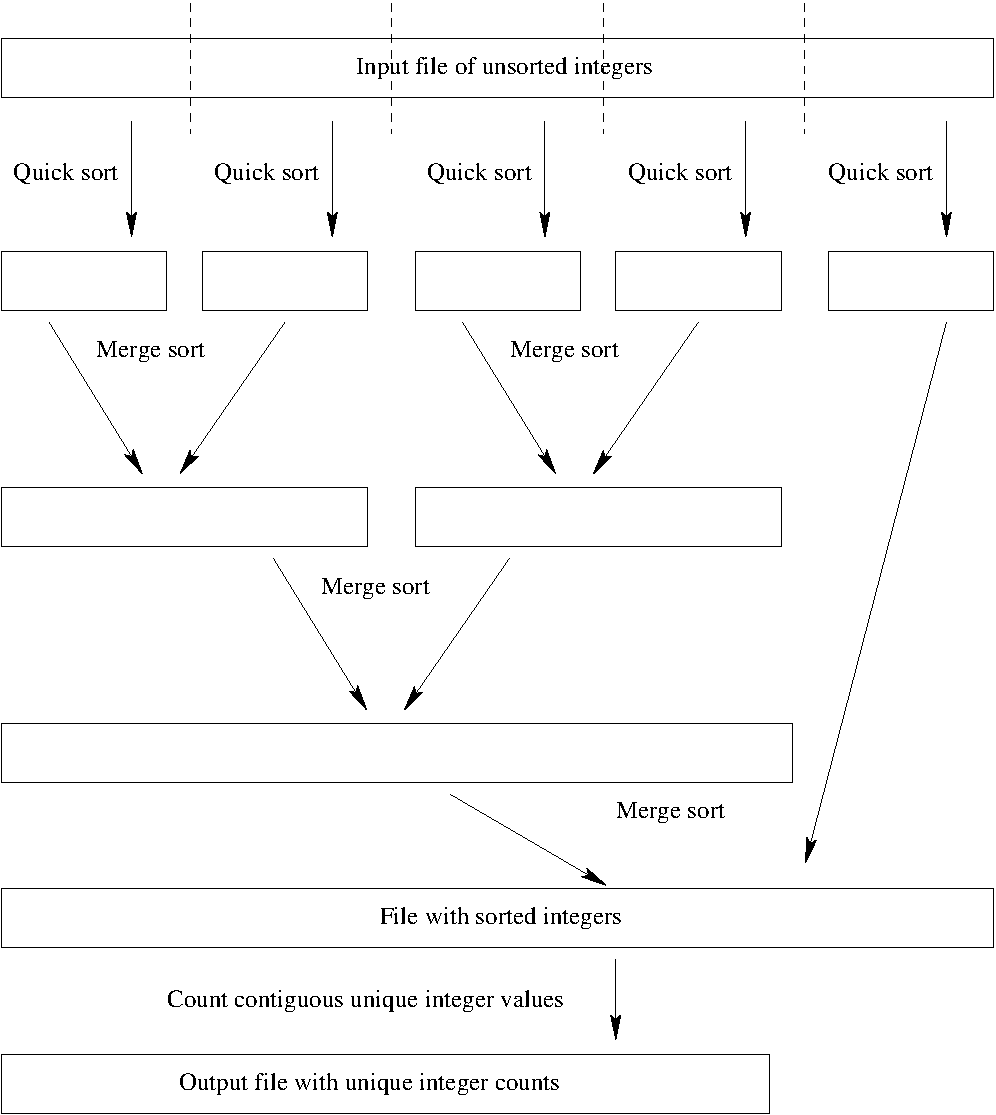
\includegraphics[width=0.9\linewidth]{count_alg.pdf}
  \caption{Histogram creation algorithm}
\end{figure}

\end{document}
%%% Local Variables: 
%%% mode: latex
%%% TeX-master: t
%%% End: 
